\chapter{Channel Coding}

%--------- Intro ---------%
\section{Overview}
This part deals with linear block codes covering their fundamental concepts, generator and parity check matrices, error-correcting capabilities, encoding and decoding, and performance analysis. The linear block code discussed in this part is Hamming code.

\subsection{Shannon's Noisy Channel Coding Theorem}
Any channel affected by noise possesses a specific “channel capacity” C a rate of conveying information that can never be exceeded without error, but in principle, an error-correcting code always exists such that information can be transmitted at rates less than C with an arbitrarily low BER.

\subsection{Channel Coding Principle}
The channel coding principle is to add redundancy to minimize error rate as illustrated in Figure~\ref{fig:channel coding principle}.
\begin{figure}[ht]
    \centering
    
\includegraphics[width= 0.8\textwidth]{au-logo-bl.PNG}
    \caption{Illustration of the channel coding principle.}
    \label{fig:channel coding principle}
\end{figure}

\subsection{Channel Coding Gain}
The bit error rate (BER) is the probability that a binary digit transmitted from the source received erroneously by the user. For required BER, the difference between the powers required for without and with coding is called the coding gain. A typical plot of BER versus Eb/No (bit energy to noise spectral density ratio) with and without channel coding is shown in Figure 2.2. It can be seen that coding can arrive at the same value of the BER at lower Eb/No than without coding. Thus, the channel coding yields coding gain which is usually measured in dB. Also, the coding gain usually increases with a decrease in BER.
\begin{figure}[ht]
    \centering
    
\includegraphics[width= 0.8\textwidth]{au-logo-bl.PNG}
    \caption{Coding gain.}
\end{figure}
%-------------------------%

%--------- Linear --------%
\section{Block Codes}
The data stream is broken into blocks of $k$ bits and each k-bit block is encoded into a block of n bits with $n > k$ bits as illustrated in Figure 2.3. The n-bit block of the channel block encoder is called the code word. The code word is formed by adding $(n - k)$ parity check bits derived from the $k$ message bits.
\begin{figure}[ht]
    \centering
    
\includegraphics[width= 0.8\textwidth]{au-logo-bl.PNG}
    \caption{Coded data stream.}
\end{figure}

\subsection*{Properties of Block Codes}

\subsubsection*{Block code rate}
The block code rate (R) is defined as the ratio of $k$ message bits and length of the code word $n$.
\[R = \frac{k}{n} \]

\subsubsection*{Code word weight}
The weight of a code word or error pattern is the number of nonzero bits in the code word or error pattern. \\
For example, the weight of a code word $c = (1, 0, 0, 1, 1, 0, 1, 0)$ is 4.

\subsubsection*{Hamming distance}
The Hamming distance between two blocks v and w is the number of coordinates in which the two blocks differ.
\[ d_{hamming}(v,w) = d(v,w) = | \{i | v_i \neq w_i, i = 0,1,\ldots,n-1 \} | \]
Example: Consider the code words $v$ = (00100) and $w$ = (10010), then the Hamming distance $d_{hamming}(v, w) = 3$. \\
Hamming distance allows for a useful characterization of the error detection and error correction capabilities of a block code as a function of the code's minimum distance.

\subsubsection*{The Minimum Distance of a Block Code}
The minimum distance of a block code $C$ is the minimum Hamming distance between all distinct pairs of code words in $C$.
\begin{GrayBox}
    \textbf{A code with minimum distance $d_{min}$ can:}
    \begin{itemize}
        \item \emph{detect} all error patterns of weight less than or equal to $(d_{min} - 1)$.
        \item \emph{correct} all error patterns of weight less than or equal to $(d_{min} - 1) / 2$.
    \end{itemize}
\end{GrayBox}
\textbf{Example:} Consider the binary code $C$ composed of the following four code words.
\[ C = \{(00100), (10010), (01001), (11111)\} \]
Hamming distance of (00100) and (10010) = 3 \\
Hamming distance of (10010) and (01001) = 4 \\
Hamming distance of (00100) and (01001) = 3 \\
Hamming distance of (10010) and (11111) = 3 \\
Hamming distance of (00100) and (11111) = 4 \\
Hamming distance of (01001) and (11111) = 3 \\
Therefore, the minimum distance $d_{min}$ = 3.

\subsection{Linear Block Codes}
A block code $C$ consisting of n-tuples $\{(c_0, c_1, . . . , c_{n-1})\}$ of symbols from $GF(2)$ is said to be binary linear block code if and only if $C$ forms a vector subspace over $GF(2)$. 
\begin{description}
    \item[Note:] finite fields are also called Galois fields (GF).
\end{description}
The code word is said to be systematic linear code word if each of the $2^k$ code words is represented as linear combination of $k$ linearly independent code words.

\subsubsection{Linear Block Codes Properties}
There are \emph{two important properties} of linear block codes which are:
\begin{description}
    \item[Property 1:] The linear combination of any set of code words is a code word.
    \item[Property 2:] The minimum distance of a linear block code is equal to the minimum weight of any nonzero word in the code.
\end{description}
Also, there are 2 well-known bounds on the minimum distance which are
\begin{description}
    \item[Singleton Bound:]
    The minimum distance of an $(n, k)$ linear code is bounded by
    \begin{equation}
        \label{eq:Singleton Bound}
        d_{min} \leq n-k+1
    \end{equation}
    \item[Hamming Bound:]
    An $(n, k)$ block code can \emph{detect} $t_{ed}$ errors per code word and can correct up to $t_{ec}$ errors per code word, provided that $n$ and $k$ satisfy the Hamming bound.
    \begin{equation}
        \label{eq:Hamming Bound}
        2^{n-k} \geq \sum_{i = 0}^{t_{ec}} \binom{n}{i} \quad \text{where} \quad \binom{n}{i} = \frac{n!}{(n-1)!i!}
    \end{equation}
    \[ t_{ec} = \frac{(d_{min} - 1)}{2} \quad , \quad t_{ed} = d_{min} - 1  \]
    The relation is the upper bound on $d_{min}$ and is known as \emph{the Hamming bound}.
\end{description}
 
\subsection{Generator \& Parity Check Matrices}
Let $\{g_0, g_1, \ldots  , g_{k-1}\}$ be a basis of code words for the $(n, k)$ linear block code $C$ and $m = [m_0, m_1, \ldots , m_{k-1}]$ the message to be encoded. The Theorem that says the code word $c = (c_0, c_1, \ldots , c_{n-1})$ for the message is uniquely represented by the following linear combination of $g_0, g_1, \ldots , g_{k-1}$
\[ c = m_0g_0 + \ldots + m_{k-1}g_{k-1} \]

for every code word $c \in C$.\\
Since every linear combination of the basis elements must also be a code word, there is a one-to-one mapping between the set of k-bit blocks $(a_0, a_1, \ldots , a_{k-1})$ over $GF(2)$ and the code words in $C$. A matrix $G$ is constructed by taking the vectors in the basis as its rows.
\[ G = \left[ \begin{array}{c}
    g_0 \\
    g_1 \\
    \vdots \\
    g_{k-1}
\end{array} \right] = \left[ \begin{array}{c c c c}
    g_{0,0} & g_{0,1} & \ldots & g_{0,n-1} \\
    g_{1,0} & g_{1,1} & \ldots & g_{1,n-1} \\
    \vdots & \vdots & \ddots & \vdots \\
    g_{k-1,0} & g_{k-1,1} & \ldots & g_{k-1,n-1}
\end{array} \right]
\]
This matrix $G$ is a generator matrix for the code $C$. It can be used to directly encode k-bit blocks in the following manner:
\[
mG = [m_0, m_1, \ldots, m_{k-1}] \cdot \left[ \begin{array}{c}
    g_0 \\
    g_1 \\
    \vdots \\
    g_{k-1}
\end{array} \right] = m_0g_0 + m_1g_1 + \ldots + m_{k-1}g_{k-1} = c
\]

The dual space of a linear block code $C$ is the dual code of $C$ and a basis $\{h_0, h_1, \ldots , h_{n-k-1}\}$ can be found for dual code of $C$, and the following parity check matrix can be constructed:
\[
H = \left[ \begin{array}{c}
    h_0 \\
    h_1 \\
    \vdots \\
    h_{n-k-1}
\end{array} \right] = \left[ \begin{array}{c c c c}
    h_{0,0} & h_{0,1} & \ldots & h_{0,n-1} \\
    h_{1,0} & h_{1,1} & \ldots & h_{1,n-1} \\
    \vdots & \vdots & \ddots & \vdots \\
    h_{n-k-1,0} & g_{n-k-1,1} & \ldots & g_{n-k-1,n-1}
\end{array} \right]
\]

In a systematic linear block code, the last $k$ bits of the codeword are \emph{the message bits}, that is
\[ c_i = m_{i-(n-k)} \quad , \quad i = n-k, \ldots , n-1 \]
While the first $n-k$ bits in the codeword are check bits generated from the k message bits according to
\[ c_0 = p_{0,0} m_0 + p_{1,0} m_1 + \ldots + p_{k-1, 0} m_{k-1} \]
\[ c_1 = p_{0,1} m_0 + p_{1,1} m_1 + \ldots + p_{k-1, 1} m_{k-1} \]
\[ \vdots \]
\[ c_{n-k-1} = p_{0,n-k-1} m_0 + p_{1,n-k-1} m_1 + \ldots + p_{k-1, n-k-1} m_{k-1} \]

The above equation can be written in a matrix form as:
\begin{equation}
    \label{equation:c=mG}
    [ c_0, c_1, \ldots, c_{n-1} ] = [ m_0, m_1, \ldots, m_{k-1} ] \left[ \begin{array}{c c c c c c c}
        p_{0,0} & p_{0,1} & \cdots & p_{0,n-k-1} & 1000 & \cdots & 0 \\
        p_{1,0} & p_{1,1} & \cdots & p_{1,n-k-1} & 0100 & \cdots & 0 \\
        \vdots & \vdots & \ddots & \vdots & \vdots & \vdots & \vdots \\
        p_{k-1,0} & p_{k-1,1} & \cdots & p_{k-1,n-k-1} & 0000 & \cdots & 1 \\     
    \end{array} \right]_{k \times n}
\end{equation}
\[ \text{or} \]
\[ c = mG \]
where $G$ is the matrix on the right hand side of the equation~\ref{equation:c=mG}. \\
The $k \times n$ matrix $G$ is called a generator matrix of the code and it has the following form:
\begin{equation}
    \label{eq:G}
    G = \left[ P | I_k \right]_{k \times n}
\end{equation}

The matrix $I_k$ is the identity matrix of order $k$, and $P$ is an arbitrary $k \times n-k $ matrix. When $P$ is specified, it defines the $(n, k)$ block code completely. The parity check matrix H corresponding to the above generator matrix G can be obtained as
\[ H = \left[ I_{n-k} | P^T \right] \]
\begin{equation}
    \label{equation:H}
    H = \left[ \begin{array}{c c c c c c c}
        1000 & \cdots & 0 & p_{0,0} & p_{0,1} & \cdots & p_{0,n-k-1} \\
        0100 & \cdots & 0 & p_{1,0} & p_{1,1} & \cdots & p_{1,n-k-1} \\
        \vdots & \vdots & \vdots & \vdots & \vdots & \ddots & \vdots \\
        0000 & \cdots & 1 & p_{0,n-k-1} & p_{1,n-k-1} & \cdots & p_{k-1,n-k-1} \\     
    \end{array} \right]
\end{equation}

\newtcbtheorem[auto counter,number within=section]{theo}
  {Theorem}{fonttitle=\bfseries\upshape, fontupper=\slshape,
     arc=0mm, colback=black!5!white,colframe=black!75!white}{theorem}

\begin{theo}{Parity Check Theorem}{}
    For any $(n, k)$ linear block code $C$ with $(n-k)\times n$ parity check matrix $H$, a code word $c \in C$ is a valid code word \textbf{if and only if} $cH^{T}=0$.
    \par\noindent\dotfill \\
    \textbf{Example:}\\
    For the following generator matrix of (7,4) block code. Find the code vector for the message vector m = (1110) and check the validity of code vector generated.
    \[
    G = \left[ \begin{array}{c c c | c c c c}
        1 & 1 & 0 & 1 & 0 & 0 & 0 \\
        0 & 1 & 1 & 0 & 1 & 0 & 0 \\
        1 & 1 & 1 & 0 & 0 & 1 & 0 \\
        1 & 0 & 1 & 0 & 0 & 0 & 1 
    \end{array} \right]
    \]
    \textbf{Solution:}\\
    The code vector for the message block $m = (1110)$ is given by
    \[
    c = mG = [1 1 1 0] \cdot \left[ \begin{array}{c c c | c c c c}
        1 & 1 & 0 & 1 & 0 & 0 & 0 \\
        0 & 1 & 1 & 0 & 1 & 0 & 0 \\
        1 & 1 & 1 & 0 & 0 & 1 & 0 \\
        1 & 0 & 1 & 0 & 0 & 0 & 1 
    \end{array} \right] = [0 1 0 1 1 1 0]
    \]
    \[
    H = \left[ \begin{array}{c c c | c c c c}
        1 & 0 & 0 & 1 & 0 & 1 & 1 \\
        0 & 1 & 0 & 1 & 1 & 1 & 0 \\
        0 & 0 & 1 & 0 & 1 & 1 & 1 
    \end{array} \right]
    \]
    \[
    cH^T = [0 1 0 1 1 1 0] \cdot \left[ \begin{array}{c c c}
        1 & 0 & 0 \\
        0 & 1 & 0 \\
        0 & 0 & 1 \\
        1 & 1 & 0 \\
        0 & 1 & 1 \\
        1 & 1 & 1 \\
        1 & 0 & 1 
    \end{array} \right] = [0 0 0]
    \]
    Hence, the generated code vector is valid.
\end{theo}

\section{Hamming Codes}
Hamming code is a linear block code capable of correcting single errors having a minimum distance $d_{min} = 3$. It is very easy to construct Hamming codes. The parity check matrix $H$ (obtained in equation~\ref{equation:H}) must be chosen so that no row in $H^T$ is zero and the first $(n-k)$ rows of $H^T$ form an identity matrix and all the rows are distinct. We can select $2^{n-k}-1$ distinct rows of $H^T$.\\
Since the matrix $H^T$ has $n$ rows, for all of them to be distinct, the following inequality should be satisfied.
\[ 2^{n-k} -1 \geq n \]
Implying that
\[ (n-k) \geq \log_2(n+1) \]
\begin{equation}
    \label{eq:n geq klog}
    n \geq k + \log_2(n+1)
\end{equation}
Hence, the minimum size $n$ for the code words can be determined from equation~\ref{eq:n geq klog}. \\

\textbf{Example:} Design a Hamming code with message block size of eleven bits. \\
\textbf{Solution:} It follows from equation~\ref{eq:n geq klog} that
\[ n \geq 11 + \log_2(n+1) \]
The smallest $n$ that satisfies the above inequality is 15, and hence, we need a $(15,11)$ block code. Thus, the transpose of the parity check matrix $H$ will be $4 \times 15$ matrix. The first four rows of $H^T$ will be $I_4$ matrix. The last eleven rows are arbitrarily chosen, with the restrictions that no row is zero, and all the rows are distinct.
\begin{equation}
    \label{eq:H solution}
    H^T = \left[ \begin{array}{c c c c}
        1 & 0 & 0 & 0 \\
        0 & 1 & 0 & 0 \\
        0 & 0 & 1 & 0 \\
        0 & 0 & 0 & 1 \\
        \hline
        0 & 1 & 0 & 1 \\
        0 & 1 & 1 & 0 \\
        0 & 1 & 1 & 1 \\
        0 & 0 & 1 & 1 \\
        1 & 0 & 0 & 1 \\
        1 & 0 & 1 & 0 \\
        1 & 0 & 1 & 1 \\
        1 & 1 & 0 & 0 \\
        1 & 1 & 0 & 1 \\
        1 & 1 & 1 & 0 \\
        1 & 1 & 1 & 1
    \end{array} \right] = \left[ \begin{array}{c}
        I_{n-k} \\
        \hline
        P^T    
    \end{array} \right]
\end{equation}

Then generator matrix $G$ equals
\[
G = \left[ \begin{array}{c c c c c c c c c c c c c c c}
    0&1&0&1&1&0&0&0&0&0&0&0&0&0&0 \\
    0&1&1&0&0&1&0&0&0&0&0&0&0&0&0 \\
    0&1&1&1&0&0&1&0&0&0&0&0&0&0&0 \\
    0&0&1&1&0&0&0&1&0&0&0&0&0&0&0 \\
    1&0&0&1&0&0&0&0&1&0&0&0&0&0&0 \\
    1&0&1&0&0&0&0&0&0&1&0&0&0&0&0 \\ 
    1&0&1&1&0&0&0&0&0&0&1&0&0&0&0 \\
    1&1&0&0&0&0&0&0&0&0&0&1&0&0&0 \\
    1&1&0&1&0&0&0&0&0&0&0&0&1&0&0 \\
    1&1&1&0&0&0&0&0&0&0&0&0&0&1&0 \\
    1&1&1&1&0&0&0&0&0&0&0&0&0&0&1
\end{array} \right]
\]

\textbf{Example:} Construct parity check and generator matrices for a $(7, 4)$ Hamming code. \\
\textbf{Solution:} The parity check matrix $H$ and generator matrix $G$ for a $(7, 4)$ Hamming code are
\[
H = \left[ \begin{array}{c c c c c c c}
    1 & 0 & 0 & 1 & 0 & 1 & 1 \\
    0 & 1 & 0 & 1 & 1 & 1 & 0 \\
    0 & 0 & 1 & 0 & 1 & 1 & 1
\end{array} \right]
\]
\[
G = \left[ \begin{array}{c c c c c c c}
    1 & 1 & 0 & 1 & 0 & 0 & 0 \\
    0 & 1 & 1 & 0 & 1 & 0 & 0 \\
    1 & 1 & 1 & 0 & 0 & 1 & 0 \\
    1 & 0 & 1 & 0 & 0 & 0 & 1
\end{array} \right]
\]

\subsection{Syndrome Table Decoding}
Consider a valid code word $c$ for transmission and let $e$ be an error pattern introduced by the channel during transmission. Then, the received vector $r$ can be written as
\[ r = c + e \]
Multiplying the $r$ by the transpose of the parity check matrix gives the syndrome $S$ which can be expressed as \\
\begin{equation}
    \label{eq:Syndrome Table Decoding}
    \begin{aligned}
        S &= r \cdot H^T \\
        &= (c+e) \cdot H^T \\
        &= cH^T + eH^T\\
        &= 0 + eH^T \\ 
        &= eH^T
    \end{aligned}
\end{equation}

Thus, the syndrome vector is independent of the transmitted code word $c$ and is only a function of the error pattern $e$. Decoding is performed by computing the syndrome of a received vector, looking up the corresponding error pattern, and subtracting the error pattern from the received word. \\

\textbf{Example:} Construct a syndrome decoding table for a $(7, 4)$ Hamming code \\
\textbf{Solution:} For a $(7, 4)$ Hamming code, there are $2^{(7-4)}$ error patterns $e$ as in Table~\ref{eq:Syndrome Table Decoding}
\begin{table}[!ht]
    \centering
    \caption{Syndrome decoding table for a $(7, 4)$ Hamming code}
    \label{tbl:syndrome decoding table}
    \begin{tabular}{cc}
        \toprule
        Error Pattern $e$ & Syndrome \\
        \midrule
        0000000 & 000 \\
        1000000 & 100 \\
        0100000 & 010 \\
        0010000 & 001 \\
        0001000 & 110 \\
        0000100 & 011 \\
        0000010 & 111 \\
        0000001 & 101 \\
        \bottomrule
    \end{tabular}
\end{table}

The syndrome for $(7, 4)$ Hamming code is computed using the parity check matrix $H$ (as given in the solution~\ref{eq:H solution}) as follows
\[ S = e \cdot H^T \]
Thus, the syndrome decoding table for a $(7, 4)$ Hamming code is as in Table~\ref{tbl:syndrome decoding table}

\subsection{Hamming Codes Decoding}
Syndrome table is used to decode the Hamming codes. The syndrome table gives the syndrome value based on the simple relationship with parity check matrix. The single-error-correcting codes (i.e., Hamming codes), are decoded by using syndrome value. Consider a code word $c$ corrupted by $e$, an error pattern with a single one in the $j^{th}$ coordinate position results a received vector $r$. Let ${h_0, h_1, \ldots , h_{n-1}}$ be the set of columns of the parity check matrix $H$. When the syndrome is computed, we obtain the transposition of the $j^{th}$ column of $H$. \\
\begin{equation}
    \label{eq:hamming codes decoding}
    s = eH^T = [0, \ldots, 0,1,0, \ldots, 0] \cdot \left[ \begin{array}{c}
        h_0^T \\
        h_1^T \\
        \vdots \\
        h_{n-1}^T
    \end{array} \right] = h_j^T
\end{equation}

The above-mentioned process in equation~\ref{eq:hamming codes decoding} can be implemented using the following algorithm:
\begin{enumerate}
    \item Compute the syndrome $s$ for the received word. If $s = 0$, the received code word is the correct code word.
    \item Find the position $j$ of the column of $H$ that is the transposition of the syndrome.
    \item Complement the $j^{th}$ bit in the received codeword to obtain the corrected code word. \\
\end{enumerate}

\textbf{Example:} Decode the received vector $r = [001100011100000]$ using the $(15,11)$ parity check matrix. \\
\textbf{Solution:} \\
\[
H = \left[ \begin{array}{c c c c c c c c c c c c c c c}
    1&0&0&0&0&0&0&0&1&1&1&1&1&1&1 \\
    0&1&0&0&1&1&1&0&0&0&0&1&1&1&1 \\
    0&0&1&0&0&1&1&1&0&1&1&0&0&1&1 \\
    0&0&0&1&1&0&1&1&1&0&1&0&1&0&1    
\end{array} \right]
\] \\
The received vector is $r = [001100011100000]$ \\
The corresponding syndrome $s = r \cdot H^T$ is \\
\[s = [0011]\] \\
The syndrome is the transposition of $7^{th}$ column of $H$. Inverting the $7^{th}$ coordinate of $r$, the following code word is obtained \\
\[c = [001100001100000]\]


\section{LDPC Coding}
Low density parity check (LDPC) codes are forward error-correction codes, invented by Robert Gallager in his MIT Ph.D. dissertation, 1960. The LDPC codes are ignored for long time due to their high computational complexity and domination of highly structured algebraic block and convolutional codes for forward error correction. A number of researchers produced new irregular LDPC codes which are known as new generalizations of Gallager's LDPC codes that outperform the best turbo codes with certain practical advantages. LDPC codes have already been adopted in satellite based digital video broadcasting and long-haul optical communication standards. This chapter discusses LDPC Code Properties, construction of parity check matrix for regular and irregular LDPC codes, efficient Encoding and Decoding of LDPC Codes, performance analysis of LDPC Codes.

\subsection{LDPC Code Properties}
Low Density Parity Check (LDPC) code is a linear error-correcting code that has a parity check matrix $H$, which is sparse i.e. with less nonzero elements in each row and column. LDPC codes can be categorized into regular and irregular LDPC codes. When the parity-check matrix $H_{(n - k)\times n}$ has the same number $w_c$ of ones in each column and the same number $w_r$ of once in each row, the code is a regular ($w_c$, $w_r$). The original Gallager codes are regular binary LDPC codes. The size of $H$ is usually very large, but the density of nonzero element is very low. LDPC code of length $n$, or denoted as an (n,$w_c$, $w_r$) LDPC code. Thus, each information bit is involved with $w_c$ parity checks, and each parity check bit is involved with $w_r$ information bits.\\
For a regular code, we have $(n-k)w_r = nw_c$ thus $w_c < w_r$.
\begin{equation}
    \label{eq:code rate}
    \begin{aligned}
        \text{code rate = } & \frac{(w_r - w_c)}{w_r} && \text{If all rows are linearly independent.} \\
        & \frac{k}{n} && \text{otherwise.}
    \end{aligned}
\end{equation}
Typically, $w_c \geq 3$. A parity check matrix with minimum column weight $w_c$ will have a minimum distance $d_{min} \geq w_c + 1$. When $w_c\geq 3$, there is at least one LDPC code whose minimum distance $d_{min}$ grows linearly with the block length $n$ thus a longer code length yields a better coding gain. Most regular LDPC codes are constructed with $w_c$ and $w_r$ on the order of 3 or 4.

\subsection{Construction of Parity Check Matrix H}
\subsubsection{Random Construction of H for Regular Codes}
In this method, the transpose of regular $(n, w_c, w_r)$ parity check matrix $H$ has the form
\[H^T =\begin{bmatrix}
H_{1}^T, H_{2}^T, ....., H_{wc}^T    
\end{bmatrix}\]
The matrix $H_1$ has $n$ columns and $\frac{n}{w_r}$ rows. The $H_1$ contains a single 1 in each column and contains 1s in its ith row from column $(i - 1)w_r + 1$ to column $i w_r$. Permuting randomly the columns of $H_1$ with equal probability, the matrices $H_2$ to $H_wc$ are obtained. The parity check matrix for $(n = 20, w_c = 3, w_r = 4)$ code constructed by Gallager is given as
\[H=\left[\begin{matrix}1\ 1\ 1\ 1\ 0\ 0\ 0\ 0\ 0\ 0\ 0\ 0\ 0\ 0\ 0\ 0\ 0\ 0\ 0\ 0\\0\ 0\ 0\ 0\ 1\ 1\ 1\ 1\ 0\ 0\ 0\ 0\ 0\ 0\ 0\ 0\ 0\ 0\ 0\ 0\\0\ 0\ 0\ 0\ 0\ 0\ 0\ 0\ 1\ 1\ 1\ 1\ 0\ 0\ 0\ 0\ 0\ 0\ 0\ 0\\0\ 0\ 0\ 0\ 0\ 0\ 0\ 0\ 0\ 0\ 0\ 0\ 1\ 1\ 1\ 1\ 0\ 0\ 0\ 0\\0\ 0\ 0\ 0\ 0\ 0\ 0\ 0\ 0\ 0\ 0\ 0\ 0\ 0\ 0\ 0\ 1\ 1\ 1\ 1\\1\ 0\ 0\ 0\ 1\ 0\ 0\ 0\ 1\ 0\ 0\ 0\ 1\ 0\ 0\ 0\ 0\ 0\ 0\ 0\\0\ 1\ 0\ 0\ 0\ 1\ 0\ 0\ 0\ 1\ 0\ 0\ 0\ 0\ 0\ 0\ 1\ 0\ 0\ 0\\0\ 0\ 1\ 0\ 0\ 0\ 0\ 0\ 0\ 1\ 0\ 0\ 0\ 1\ 0\ 0\ 0\ 1\ 0\ 0\\0\ 0\ 0\ 1\ 0\ 0\ 0\ 0\ 0\ 0\ 1\ 0\ 0\ 0\ 1\ 0\ 0\ 0\ 1\ 0\\0\ 0\ 0\ 0\ 0\ 0\ 0\ 1\ 0\ 0\ 0\ 1\ 0\ 0\ 0\ 1\ 0\ 0\ 0\ 1\\1\ 0\ 0\ 0\ 0\ 1\ 0\ 0\ 0\ 0\ 0\ 1\ 0\ 0\ 0\ 0\ 0\ 1\ 0\ 0\\0\ 1\ 0\ 0\ 0\ 0\ 1\ 0\ 0\ 0\ 1\ 0\ 0\ 0\ 0\ 1\ 0\ 0\ 0\ 0\\0\ 0\ 1\ 0\ 0\ 0\ 0\ 1\ 0\ 0\ 0\ 0\ 1\ 0\ 0\ 0\ 0\ 0\ 1\ 0\\0\ 0\ 0\ 1\ 0\ 0\ 0\ 0\ 1\ 0\ 0\ 0\ 0\ 1\ 0\ 0\ 1\ 0\ 0\ 0\\0\ 0\ 0\ 0\ 1\ 0\ 0\ 0\ 0\ 1\ 0\ 0\ 0\ 0\ 1\ 0\ 0\ 0\ 0\ 1\\\end{matrix}\right]\]

\subsubsection{Algebraic Construction of H for Regular Codes}
The construction of the parity check matrix $H$ using algebraic construction as follows [2, 3]. Consider an identity matrix $I_a$ where $a > (w_c - 1)(w_r - 1)$ and obtain the following matrix by cyclically shifting the rows of the identity matrix $I_a$ by one position to the right.
\[A^1=\left[\begin{matrix}0\ 1\ 0\ 0\ .\ .\ .\ .\ .\ .\ 0\\0\ 0\ 1\ 0\ .\ .\ .\ .\ .\ .\ 0\\0\ 0\ 0\ 1\ .\ .\ .\ .\ .\ .\ 0\\0\ 0\ 0\ 0\ .\ .\ .\ .\ .\ .\ 1\\1\ 0\ 0\ 0\ .\ .\ .\ .\ .\ .\ 0\\\end{matrix}\right]\]
Defining $A^0 = I_a$ the parity check matrix $H$ can be constructed as
\[H=\left[\begin{matrix}A^0&A^0&A^0&\ldots&A^0\\A^0&A^{1\ \ }&A^2&\ldots&A^{Wr-1}\\A^0&\ A^{2\ }&\ A^4&\ldots&A^{2(Wr-1)}\\\ &\ &\ &\ldots&\ \\A^0&\ A^{\left(Wc-1\right)\ \ }&A^{2(Wc-1)}&\ldots&A^{(Wc-1)(Wr-1)}\\\end{matrix}\right]\]

The constructed $H$ matrix has $w_ca$ rows and $w_ra$ columns, and it is of a regular ($w_ra$, $w_c$, $w_r$) having the same number of $w_r$ ones in each row and the same number of $w_c$ ones in each column. It is four cycle free construction. The algebraic LDPC codes are easier for decoding than random codes. For intermediate n, well designed algebraic codes yields a low BER.

\textbf{Example:} Construct H matrix with $w_c = 2$ and $w_r = 3$ using algebraic construction method.\\
\textbf{Solution} Since $(w_c - 1)(w_r - 1) = 2$
\[A=\left[\begin{matrix}A^0&A^1&A^0\\A^0&A^0&A^1\\A^1&A^0&A^0\\\end{matrix}\right]\]
\[H=\left[\begin{matrix}A^0&A^0&A^0\\A^1&A^1&A^1\\\end{matrix}\right]=\left[\begin{matrix}1\ 0\ 0\ 1\ 0\ 0\ 1\ 0\ 0\\0\ 1\ 0\ 0\ 1\ 0\ 0\ 1\ 0\\0\ 0\ 1\ 0\ 0\ 1\ 0\ 0\ 1\\1\ 0\ 0\ 0\ 1\ 0\ 0\ 0\ 1\\0\ 1\ 0\ 0\ 0\ 1\ 1\ 0\ 0\\0\ 0\ 1\ 1\ 0\ 0\ 0\ 1\ 0\\\end{matrix}\right]\]

\subsubsection{Random Construction of H for Irregular Codes}
In the random construction of the parity check matrix $H$ , the matrix is filled with ones and zeros randomly satisfying LDPC properties.\\
An example of parity check matrix for irregular LDPC code is
\[H=\left[\begin{matrix}1\ 1\ 0\ 1\ 1\ 0\ 0\ 1\ 0\ 0\\0\ 1\ 1\ 0\ 1\ 1\ 0\ 0\ 0\ 0\\0\ 0\ 0\ 1\ 0\ 0\ 0\ 1\ 1\ 1\\1\ 1\ 0\ 0\ 0\ 1\ 1\ 0\ 1\ 0\\0\ 0\ 1\ 0\ 0\ 1\ 0\ 1\ 0\ 1\\\end{matrix}\right]\]

\subsubsection{Representation of Parity Check Matrix Using Tanner Graphs}

The Tanner graph of the parity check matrix $H$ is a bipartite graph. It has bit nodes or variable nodes (VN) equal to the number of columns of $H$ , and check nodes (CN) equal to the number of rows of $H$. If $H_{ji}= 1$, i.e. if variable $i$ participates in the $j^{th}$ parity-check constraint, then check node $j$ is connected to variable node $i$.

\textbf{Example:} Construct Tanner graph for the following parity check matrix
\[H=\left[\begin{matrix}1\ 1\ 0\ 0\ 1\ 1\ 1\ 1\ 0\ 0\\1\ 0\ 1\ 1\ 0\ 1\ 0\ 1\ 0\ 1\\0\ 1\ 0\ 1\ 1\ 0\ 0\ 1\ 1\ 1\\1\ 0\ 1\ 0\ 1\ 0\ 1\ 0\ 1\ 1\\0\ 1\ 1\ 1\ 0\ 1\ 1\ 0\ 1\ 0\\\end{matrix}\right]\]
\textbf{Solution} The $H$ matrix has 10 columns and 5 rows. Hence, the associated tanner graph with 10 bit nodes and 5 check nodes is shown in Figure~\ref{fig:Tanner graph}.
\begin{figure}[h]
\centering
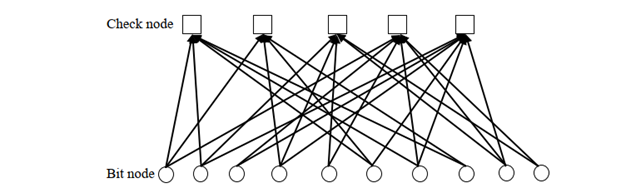
\includegraphics[width=6.47 in, height=2.01in]{27.PNG}
\caption{Tanner graph of $H$ matrix of the above example.}
\label{fig:Tanner graph}
\end{figure}

\subsection{LDPC Encoding}
\subsubsection{Preprocessing Method}
For coding purposes, we may derive a generator matrix $G$ from the parity check matrix $H$ for LDPC codes by means of Gaussian elimination in modulo-2 arithmetic. Since the matrix $G$ is generated once for a parity check matrix, it is usable in all encoding of messages. As such this method can be viewed as the preprocessing method. $1 \times n$ code vector $c$ is first partitioned as
\[C = [b : m]\]
where $m$ is $1 \times k$ message vector, and $b$ is the $1 \times n-k$ parity vector correspondingly, the parity check matrix $H$ is partitioned as
\[H^T=\left[\begin{matrix}H_1\\\ldots\\H_2\\\end{matrix}\right]\]
where $H_1$ is a square matrix of dimensions $(n - k)\times (n - k)$, and $H_2$ is a rectangular matrix of dimensions $k\times (n- k)$ transposition symbolized by the superscript T is used in the partitioning of matrix $H$ or convenience of representation. \\
Imposing the constraint $C H^T = 0$. \\
We may write
\[\left[b\ :\ m\right]\left[\begin{matrix}H_1\\ \ldots\\H_2\\\end{matrix}\right]=0\]
or equivalently
\[bH_1 + m H_2 = 0\]
The vectors $m$ and $b$ are related by
\[b = m P\]
where $P$ is the coefficient matrix. For any nonzero message vector $m$, the coefficient matrix of LDPC codes satisfies the condition
\[P H_1 + H_2 = 0\]
Which holds for all nonzero message vectors and, in particular, in the form $[0, \ldots, 0, 1, 0, \ldots, 0]$ that will isolate individual rows of the generator matrix. Solving the above Equation for matrix $P$, we get
\[P = H_2 H_{1}^{-1}\] 
where $H_{1}^{-1}$ is the inverse matrix of $H_1$, which is naturally defined in modulo-2 arithmetic. Finally, the generator matrix of LDPC codes is defined by
\[G = [P : I_k ] = [H_2 H_{1}^{-1} : I_k ]\]
where $I_k$ is the $k \times k$ identity matrix. The codeword can be generated as
\[C = mG\]

\textbf{Example:} Construct generator matrix $G$ for the following $(10, 3, 5)$ regular parity check matrix.
\[\left[\begin{matrix}1\ 1\ 0\ 1\ 0\ 1&\vdots&0\ 0\ 1\ 0\\0\ 1\ 1\ 0\ 1\ 0&\vdots&1\ 1\ 0\ 0\\1\ 0\ 0\ 0\ 1\ 1&\vdots&0\ 0\ 1\ 1\\0\ 1\ 1\ 1\ 0\ 1&\vdots&1\ 0\ 0\ 0\\1\ 0\ 1\ 0\ 1\ 0&\vdots&0\ 1\ 0\ 1\\0\ 0\ 0\ 1\ 0\ 0&\vdots&1\ 1\ 1\ 1\\\end{matrix}\right]\]
\textbf{Solution:}
\[H_1=\left[\begin{matrix}1\ 0\ 1\ 0\ 1\ 0\\1\ 1\ 0\ 1\ 0\ 0\\0\ 1\ 0\ 1\ 1\ 0\\1\ 0\ 0\ 1\ 0\ 1\\0\ 1\ 1\ 0\ 1\ 0\\1\ 0\ 1\ 1\ 0\ 0\\\end{matrix}\right]\ \ H_2=\left[\begin{matrix}0\ 1\ 0\ 1\ 0\ 1\\0\ 1\ 0\ 0\ 1\ 1\\1\ 0\ 1\ 0\ 0\ 1\\0\ 0\ 1\ 0\ 1\ 1\\\end{matrix}\right]\ \ \] 
\[H_1^{-1}=\left[\begin{matrix}0\ 0\ 1\ 0\ 1\ 1\\1\ 0\ 1\ 0\ 0\ 1\\1\ 1\ 1\ 0\ 0\ 0\\1\ 1\ 0\ 0\ 1\ 0\\0\ 1\ 0\ 0\ 1\ 1\\1\ 1\ 1\ 1\ 0\ 1\\\end{matrix}\right]\ \ \ \ \]
\[H_2H_1^{-1}=\left[\begin{matrix}0\ 1\ 0\ 1\ 0\ 1\\0\ 1\ 0\ 0\ 1\ 1\\1\ 0\ 1\ 0\ 0\ 1\\0\ 0\ 1\ 0\ 1\ 1\\\end{matrix}\right]\left[\begin{matrix}0\ 0\ 1\ 0\ 1\ 1\\1\ 0\ 1\ 0\ 0\ 1\\1\ 1\ 1\ 0\ 0\ 0\\1\ 1\ 0\ 0\ 1\ 0\\0\ 1\ 0\ 0\ 1\ 1\\1\ 1\ 1\ 1\ 0\ 1\\\end{matrix}\right]=\left[\begin{matrix}1\ 0\ 0\ 1\ 1\ 0\\0\ 0\ 0\ 1\ 1\ 1\\0\ 0\ 1\ 1\ 1\ 1\\0\ 1\ 0\ 1\ 1\ 0\\\end{matrix}\right]\ \ \ \ \ \]
The generator matrix
\[G = [H_2 H_{1}^{-1} : I_k ] =\left[\begin{matrix}1\ 0\ 0\ 1\ 1\ 0\ \vdots1\ 0\ 0\ 0\\0\ 0\ 0\ 1\ 1\ 1\ \vdots0\ 1\ 0\ 0\\0\ 0\ 1\ 1\ 1\ 1\ \vdots0\ 0\ 1\ 0\\0\ 1\ 0\ 1\ 1\ 0\ \vdots0\ 0\ 0\ 1\\\end{matrix}\right] \]

\subsection{LDPC in 5G NR standards} 
Low-Density Parity-Check (LDPC) codes are linear error-correcting codes. According to the 3rd Generation Partnership Project (3GPP) TS 38.212, two channel coding codes, i.e., Polar codes and LDPC codes, are recommended for the Fifth-generation (5G) New Radio (NR). Polar codes are applied to 5G NR control channels. LDPC codes are suitable for 5G NR shared channels due to its high throughput, low latency, low decoding complexity and rate compatibility. \\
LDPC codes can be used to different block sizes with varying code rates because of the design of rate-compatible base graphs. Another advantage of 5G NR LDPC codes is that the performance of LDPC codes has an error floor around or below block error rate (BLER) 10-5 for all code sizes and code rates. \\
So LDPC codes play an important role in channel coding for 5G communication. Gallager invented LDPC codes in 1962 . \\
LDPC codes are linear block codes based on sparse parity-check matrix. It is forgotten for dozens of years because of the limited computation ability. In recent years, LDPC codes attract more attention because of their efficient decoding algorithms, excellent error-correcting capability, and their performance close to the Shannon limit for large code lengths. 5G needs to support high throughput up to 20 Gbps and a wide range of block sizes with different code rates for the data channels and hybrid automatic repeat request (HARQ). LDPC codes can fulfil the requirements. The base graphs defined in 3GPP TS 38.212 are structured parity-check matrix, which can efficiently support HARQ and rate compatibility that can support arbitrary amount of transmitted information bits with variable code rates. \\

LDPC plays a vital role in 5G NR. 5G technology has changed the way of people living in many aspects. We must build a digital trust society and comply with ethical requirements.
5G technology can help to reduce carbon emissions, as well as enable innovative applications in a range of sectors, from smart grid to precision agriculture, thereby helping to reduce CO2 emissions.

\subsubsection{Goals} 
The general objective of this part is to develop LDPC encoding and decoding chains, optimize LDPC encoding and decoding algorithms for implementing them on 5G. The specific objectives are to:
\begin{itemize}
    \item Understand the existing link level simulation code from 5G.
    \item Develop LDPC encoding and decoding chains according to 3GPP specification.
    \item Explore efficient LDPC encoding algorithm.
    \item Explore different LDPC decoding techniques.
    \item Optimize LDPC decoding algorithms for 5G NR shared channels.
    \item Implement optimized LDPC decoding algorithms on 5G.
    \item Evaluate the performance of algorithms in terms of BLER v.s. SNR graphs and execution CPU time.
    \item Discuss the benefits and drawbacks of the studied LDPC decoding algorithms with different code block sizes.
\end{itemize}

\subsubsection{NR Base graphs and parity-check matrix}
\textbf{Base graphs analysis}
In 3GPP TS 38.212 standard, there are two kinds of base graphs and their usage are determined by code rate and size of information bits. 
\begin{description}
    \item[Base graph 1:] 46 rows and 68 columns.
    \[K = 22Zc\]
    \item[Base graph 2:] 42 rows and 52 columns.
    \[K = 10Zc\]
\end{description}
Where $K$ is the maximum number of information bits, and $Z_c$ is the lifting size (expansion factor) shown Figure~\ref{fig:ldpc lifting sizes}. There are 51 lifting sizes from 2 to 384 for each base graph.
\begin{tabularx}{0.8\textwidth} { | m{1em} | m{1cm}| m{1cm} | m{1em} | m{1cm}| m{1cm} | m{1em} | m{1cm}| m{1cm} | } 
    \hline
    $i_{LS}$ & 0 & 1 & 2 & 3 & 4 & 5 & 6 & 7 \\
    \hline
    a & 2 & 3 & 5 & 7 & 9 & 11 & 13 & 15 \\
    \hline
    $j_a$ & 7 & 7 & 6 & 5 & 5 & 5 & 4 & 4 \\
    \hline
\end{tabularx}
\[Z_c = a.2^j     , j = 0,...., j_a\]

\begin{figure}[h]
\centering
\label{fig:ldpc lifting sizes}
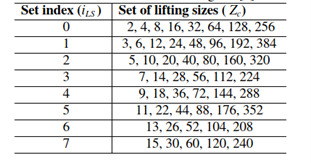
\includegraphics[width=3.24 in, height=1.7in]{28.PNG}
\caption{Table sets of LDPC lifting size}
\end{figure}

Both base graph 1 and base graph 2 have the same block structure shown in Figure~\ref{fig:block structure}. The columns include information columns, core parity columns, and extension parity columns. The rows are divided into core check rows and extension check rows.

\begin{figure}[h]
\centering
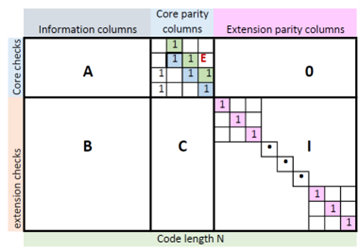
\includegraphics[width=3.75 in, height=2.6in]{29.PNG}
\caption{Base graphs block structure}
\label{fig:block structure}
\end{figure}

For base graph 1:
$A$ is a $4 \times 22$ matrix \\
$E$ is a $4 \times 4$ matrix \\
$0$ is $4 \times 42$ all zero matrix \\
$B$ is a $42 \times 22$ matrix \\
$C$ is a $42 \times 4$ matrix \\
$I$ is $42 \times 42$ identity matrix. \\

For base graph 2: \\
$A$ is a $4 \times 10$ matrix \\
$E$ is a $4 \times 4$ matrix \\
$0$ is $4 \times 38$ all zero matrix\\
$B$ is a $38 \times 10$ matrix \\
$C$ is a $38 \times 4$ matrix \\
$I$ is $38 \times 38$ identity matrix. \\

Sub-matrix E is a double diagonal matrix that is benefit for encoding. \\
An example of base graph 1 with set index iLS = 1 in 3GPP TS 38.212 standard is shown in Figure~\ref{fig:standard base graph 1}. In order to distinguish with the number 1 in base graphs in 3GPP TS 38.212 standard, -1 value in the base graph will be replaced by NULLS.

\begin{figure}[h]
\centering
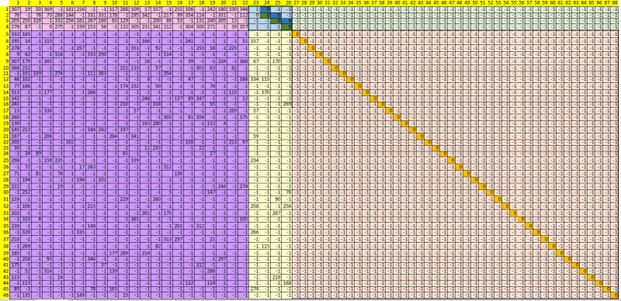
\includegraphics[width=6.47 in, height=3.14in]{30.PNG}
\caption{Base graph 1 with iLS = 1}
\label{fig:standard base graph 1}
\end{figure}

In 3GPP TS 38.212 standard, the base graphs correspond to maximum lifting size for each set index $i_LS$ shown in Figure~\ref{fig:ldpc lifting sizes}. For example, the base graph shown in Figure~\ref{fig:standard base graph 1} is the base graph with lifting size 384 corresponding to index $i_LS = 1$. The value of each element $P_i$, $j$ also known as circular shift value is from -1 to 383, which is a property of the base graph. The property is that circular shift value $P_{i,j}$ for base graph with arbitrary lifting size $Z_c$ ranges from $-1$ to $Z_c - 1$.

\textbf{Parity-check matrix calculation} \\
The parity-check matrix $H$ is obtained by replacing each element of base graph $H_BG$ with a $Z_c \times Z_c$ matrix, according to the following rules:
\begin{itemize}
    \item Each element of value $-1$ in $H_BG$ is replaced by an all zero matrix of size $Z_c \times Z_c$
    \item Each element of value $0$ in $H_BG$ is replaced by an identity matrix of size $Z_c \times Z_c$
    \item Each element of value from $1$ to $Z_c - 1$ in $H_BG$ which is denoted by $P_i$, $j$ is replaced by a circular permutation matrix $I$$(P_{i,j})$ of size $Z_c \times Z_c$, where $i$ and $j$ are the row and column indices of the element, and $I$$(P_{i,j})$ is obtained by circularly shifting the identity matrix $I$ of size $Z_c \times Z_c$ to the right $(V_{i,j})$ times. The main advantage of using a circularly shifting identity matrix is that it can reduce the memory requirement for implementation while also can facilitate the use of a simple switch network for encoding and decoding.
\end{itemize}

To simplify, a small example was used to explain the principle of how to get parity-check matrix $H$ (Figure~\ref{fig:H parity}). Assume that $B$ (Figure~\ref{fig:B}) is a base graph with lifting size 4.

\begin{figure}[h]
\centering
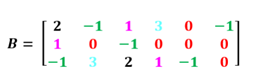
\includegraphics[width=2.65 in, height=0.82in]{31.PNG}
\caption{Base graph B}
\label{fig:B}
\end{figure}

\begin{figure}[h]
\centering
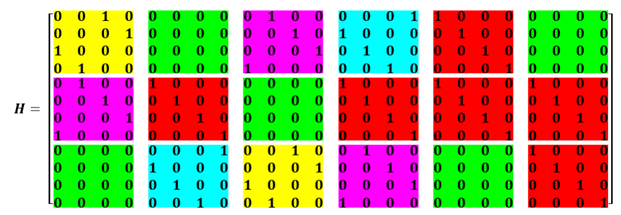
\includegraphics[width=6.47 in, height=2.24in]{32.PNG}
\caption{Parity-check matrix H}
\label{fig:H parity}
\end{figure}

\subsubsection{LDPC channel coding chain}
3GPP TS 38.212 standard defines the LDPC channel coding chain before the encoded information bits transmitted through the channel model. It is called LDPC encoding chain including 6 parts for both PUSCH and PDSCH. Figure~\ref{fig:coding chain} shows the LDPC encoding chain, which includes transport block CRC attachment, LDPC base graph selection, code block segmentation and code block CRC attachment, LDPC encoding, rate matching and code block concatenation. 

\begin{figure}[h]
\centering
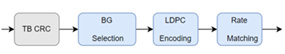
\includegraphics[width=3.95 in, height=0.75in]{33.PNG}
\caption{LDPC channel coding chain}
\label{fig:coding chain}
\end{figure}

\subsubsection{LDPC base graph selection}
LDPC base graph is selected based on the size of transport block (TB) message $A$ and transport block coding rate $R$. \\
If $A \leq 292$ , or if $A \leq 3824$ and $R \leq 0.67$ , or if $R \leq 0.25$ , LDPC base graph 2 is used. 
Otherwise, LDPC base graph 1 is used.

\subsection{Rate matching}
The purpose of rate matching is to adapt different code rates
Rate matching is carried out on each code block independently. Assume that the input message to the $r_{th}$ code block is $d_1, d_2, \ldots , d_N$, where $N = 66Z_c$ for base graph 1 and $N = 50Z_c$ for base graph 2. $E_r$ is the length of rate matching output message of the $r_{th}$ code block. The output message after rate matching of the $r_{th}$ code block is $e_1, e_2, \ldots , e_{Er}$ which is calculated using equation
\[e_k = d_k, if d_k \neq NULL, where  1 \leq k \leq Er\] 

In our project we make rate matching by puncturing as follows
\begin{equation}
    \label{eq:rate}
    \begin{aligned}
        R = & \frac{K}{n} \\
        = & \frac{K_bZ_c}{n_bZ_c} \\
        = & \frac{K_b}{n_b} \\
        K_b = & n_b - m_b
    \end{aligned}
\end{equation}

\begin{description}
    \item[$K_b$:] message bits(for base graph)
    \item[$n_b$:] code word length (for base graph) = columns of base graph
\end{description}
 
New columns after rate matching:
\begin{equation}
    \label{eq:New columns after rate matching}
    n_{bRM}=\left\lceil\frac{K_b}{R}\right\rceil
\end{equation}
New rows after rate matching:
\begin{equation}
    \label{eq:New rowa after rate matching}
    m_{bRM}=n_{bRM}-K_b
\end{equation}